\section{Backgrounds}
\label{sect:bkg}
We separate the backgrounds into two distinct categories.  Those with 
``fake'' \Tau, i.e., events where a quark or gluon jet has been misidentified
as a \Tau, and those without \Tau misidentifications.  
The fake \Tau backgrounds arise mostly from QCD and \wjets events.  The 
other backgrounds are from \ttbar, $Z+$ jets, dibosons, and Higgs decays.
Backgrounds with fake \Tau are estimated with data-driven methods; the 
remaining backgrounds are taken from Monte Carlo. The main backgrounds
are discussed here, but the others are very small, so they are dropped from the 
discussion.

%In different channels, the contribution of the events with a fake \Tau, namely QCD and \wjets is estimated using the data. 
%For the prompt \Tau's, from top, $\cPZ$jets, di-boson and higgs we trust 
%the MC, but the important contributions are validated in a signal like region. 
%In this section we will discuss the different background estimation techniques used.
%In continue, estimation of different backgrounds are explained.

\subsection{\texorpdfstring{QCD background estimation in the $\tauTau$ channel}{QCD background estimation in the tau-tau channel}}
\label{sect:bkgQCD}
Events from QCD can enter the signal regions if two quark or gluon jets are 
misidentified as \Tau, and the rest of the kinematical selections are also 
satisfied.  Isolation is an important 
discriminant between fake \Tau and prompt \Tau.
Therefore we define control regions in the 
\Tau pair isolation vs. \mttwo or \SumMT 
planes, as shown in Fig.~\ref{fig:ABCDQCD}. We then estimate the QCD background
in the signal regions starting from the event counts in the
control regions under the assumption
that for fake \tauTau the isolation is uncorrelated with \mttwo or \SumMT.
This assumption was checked in the QCD dominated region of data.
%{\bf (Not clear to me what isolation means here, because
%you have two \Tau and therefore two isolations.  Which of the 
%two isolations do you actually use?  This needs to be specified).}

To reduce contamination from prompt \tauTau, in the control regions with at least one loose \Tau, 
the same-sign pairs are selected.  Residual contributions from prompt
\tauTau and \wjets are subtracted off based on Monte Carlo expectations.
In addition, the requirement on $\Delta \Phi$
is removed to improve on the statistical power of the method. 
The final estimate of the background
is taken from the control regions extrapolation with corrections
associated with the same-sign requirement and the efficiency of 
the $\Delta \Phi$ requirement for QCD events.


%Due to the large cross section of the QCD multijet events and lack of the statistics, there is a large statistical uncertainty on the 
%yield of the QCD events from MC. On the other hand, 
%The QCD multijet events contribute to the signal selection of the \tauTau channel, when two jets are 
%fakely identified as \Tau's. The fake rate can be different between data and MC, so a data driven method is developed to estimate the 
%contribution of the QCD multijet events. 
%Since the search variable (\mttwo in \binone and \SumMT in \bintwo) and the 
%isolation of the \Tau's are uncorrelated in the QCD events, the ratio of the events selected by the signal cuts over the events 
%with loosely isolated \Tau's should be independent from the search variable, so one can find the ratio in the low \mttwo or \SumMT and 
%multiply it to the number of events in the control region which is defined same as the signal region except the \Tau's are loosely isolated. 
%This would give an estimate of the QCD events in the signal region. In the signal region, loosely isolated  \Tau's 
%($I_{\Tau} <$ 2 \GeV ) 
%are excluded, but in the control region, only the pairs with at least one loosely isolated \Tau are selected. 
%These pairs are requested to be same-sign to suppress the signal contamination. To further increase the statistics 
%in different regions, the cut on the minimum angle in the transverse plane between the \MET and the jets is removed. The final estimation
%is corrected by the efficiency of this cut which is read from data and will be described in continue.

%{\bf It seems to me that this procedure would at the same time estimate 
%the \wjets background with one real \Tau and one fake \Tau. (??)}


\begin{figure}[!Hhtb]
\centering
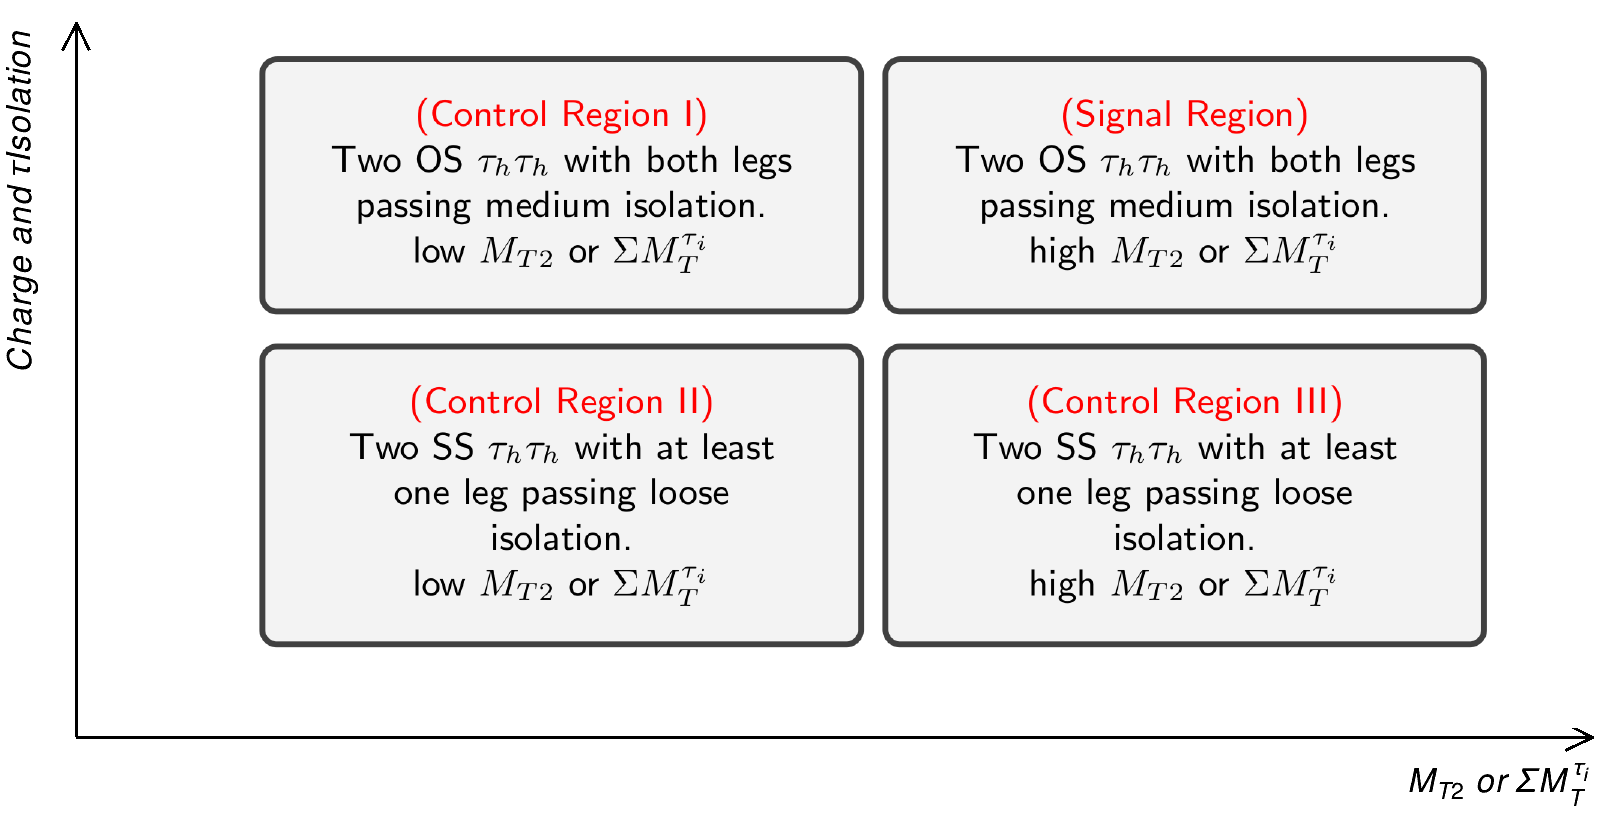
\includegraphics[angle=0,scale=0.30]{Bkg/ABCD.png}
\caption{Schematic description of the regions used to estimate the QCD backgrounds.}
\label{fig:ABCDQCD}
\end{figure}

%Non-QCD events from MC are subtracted from data to find a QCD sample.
%In the low \mttwo or \SumMT of the QCD sample, the ratio of the signal like events over the same-sign loose pairs 
%is found and verified to be flat as a function of the search variable. 
%A horizontal line is fitted to
%This ratio is multiplied to the same-sign loose pairs in high \mttwo or \SumMT and corrected by the efficiency of the 
%cut on the minimum angle between the \MET and the jets, to find the QCD contamination in the signal region. 
%The efficiency of the cut on the minimum angle between the \MET and the jets, is found with the same events as a function of the search variables.
%The value of the efficiency in the last bin in vicinity of the signal region is used to correct the estimation.
%To estimate the systematic uncertainty of the estimated value and take into account the potential correlation between the two values, 
%the method to extract the
%ratio and the efficiency are varied from approximating by a flat line to fitting by a straight line with a floating slope 
%or using the value of the  last bin before the signal region. 
%This is  also a measure  of the correlation between the two variables which are assumed to be uncorrelated. 


\begin{table}[!Hhtb]
\begin{center}
\begin{tabular}{|l|c|}
\hline\hline
 Region      &  Estimation\\
\hline\hline
%SR1      & 0.15 $\pm$ 0.22 $\pm$ 0.13 \\   
SR1      & 0.13 $\pm$ 0.19 $\pm$ 0.10 \\
\hline
%SR2      & 0.82 $\pm$ 0.65 $\pm$ 0.07  \\
SR2      & 1.15 $\pm$ 0.81 $\pm$ 0.25  \\
\hline\hline
\end{tabular}
\caption{The estimated QCD background in the \tauTau channel. The first uncertainty is statistical and systematic of the method, the second is systematic due to correlation assumptions.}
\label{4QCDbg}
\end{center}
\end{table}

Table \ref{4QCDbg} 
summarizes the estimation of the QCD background contribution in the two signal regions after extrapolation from the control regions and 
correcting for the $\Delta \Phi$ efficiency.  
The systematic uncertainties are associated with the uncertainty on the validity 
of the assumption that isolation and \mttwo or \SumMT are not correlated.
%${\bf (I think that this is what you had in the original text,
%but what about the efficiency of the $\Delta \Phi$ requirement and the 
%same-sign vs. opposite-sign business?)}


\subsection{\texorpdfstring{\wjets background estimation in the $\tauTau$ channel}{Wjets background estimation in the tau-tau channel}}
\label{sect:bkgW}
The contribution of the \wjets background in \tauTau channels is taken from simulation where the simulation of this process is validated in a data control sample. 
%While in SR2 region the number of simulated \wjets events is large enough to provide a reliable estimate, 
In different signal regions after the final requirement of \mttwo $>$ 90 \GeV or \SumMT $>$ 250 \GeV, the number of the Monte Carlo events for \wjets sample is very low and the 
predicted value is not reliable. 
Therefore, a valid estimation is necessary for the efficiency of the final requirement with respect to the preselection condition, % of \mttwo $>$ 40 \GeV, 
$\epsilon_{\rm M_{T2}}=\frac{N_{\rm M_{T2}>90}}{N_{\rm M_{T2}>40}}$ for  \binone and $\epsilon_{\SumMT}=\frac{N_{\SumMT>250}}{N_{40<\rm M_{T2}<90}}$ for \bintwo. In continue, this efficiency of the Final Selection is shown as $\epsilon_{FS}$.

Since the size of the simulated \wjets sample is not large enough to adequately populate our desired phase space, %$\epsilon_{\rm M_{T2}}$ 
$\epsilon_{FS}$ is calculated in a phase space with looser selection criteria. It is first evaluated in a \wjets sample with a pair of opposite-charge \Tau's where the \Tau candidates are selected similar to those in signal region. 
%Events in this sample are required to also meet the $\mttwo>40\,\GeV$ criterion. 
Additional signal selection requirements, such as $\Delta \Phi$ or lepton veto, are applied one by one such that two orthogonal subsamples (passing and failing) are obtained. The $\epsilon_{FS}$ quantity is calculated in all subsamples. The values are found to be compatible within the statistical uncertainties; their weighted average is taken as the final estimate for $\epsilon_{FS}$ with weights corresponding to the size of the simulated sample at each step. The uncertainty on the \Tau energy scale introduces the largest variation on $\epsilon_{FS}$. This variation is considered as a systematic uncertainty on the estimated efficiency.

Since the \wjets contamination is estimated from simulation, one needs to further verify the overall normalization as well as the $\epsilon_{FS}$ estimation in data. The control sample used for such validation is constructed based on the \muTau signal selection requirements. The selected \muTau pair in this region is required to be same-sign with a less strict \Tau isolation condition. Moreover, jets fulfilling the loose b jet identification criteria are vetoed, \tauMT requirement is removed and the \mttwo (\SumMT) requirement is changed to $40<\mttwo<60\,\GeV$ ($120<\SumMT<220\,\GeV$). The \wjets events constitute more than 90\% of this control sample and the overall normalization from simulation is consistent with data, within uncertainties.

To check the data-simulation compatibility for the $\epsilon_{FS}$ estimate, %the \mttwo condition is modified to $\mttwo>40\,\GeV$. The contribution of \wjets events remains almost unchanged. 
the same control sample is used. The $\epsilon_{FS}$ quantity is evaluated in data and simulation and the data-to-simulation ratio is used to correct the $\epsilon_{FS}$ estimation in signal region. The difference between the predicted and measured $\epsilon_{FS}$ is taken into account as an additional uncertainty. 

%The final value for the contribution of \wjets in this signal region is $0.69\pm0.54$.
Table \ref{tbl:Wbkg} summarizes the results of  the method for different signal regions of the \tauTau channel.
\begin{table}[!Hhtb]
\begin{center}
\begin{tabular}{lc}
\hline\hline
Signal Region & \wjets Estimation Results\\
\hline
\tauTau \binone & 0.69 $\pm$ 0.13 (stat.) $\pm$ 0.14 (sys. fit) $\pm$ 0.52 (sys. shape)\\
\tauTau \bintwo & 2.70 $\pm$ 0.22 (stat.) $\pm$ 0.71 (sys. fit) $\pm$ 0.68 (sys. shape)\\
\hline\hline
\end{tabular}
\caption{The \wjets estimation results in both search regions. The systematics due to the fit comes from the maximum
variation of the estimation found from up and down scaled samples with respect to the nominal one.
 The ``sys. shape''
takes into account the difference between the shape of the search variable distribution in data and Monte Carlo.}
\label{tbl:Wbkg}
\end{center}
\end{table}

%In \binone of the \tauTau channel, the number of remaining events for \wjets from MC is zero, but it has a large statistical uncertainty due to lack of the statistics in the simulated sample. To have a better estimation of the Wjets contribution in the final yields, the yield before the last cut (\mttwo $>$ 90 \GeV) is multiplied by the efficiency of the cut. To find the efficiency, several cuts like lepton veto, \Z veto and the minimum angle in the transverse plane between the \MET and the jets are relaxed to have a high statistics sample. The cut efficiency is found in the exclusive samples that either fail or pass each relaxed cut to remove any correlation between the cuts and the \mttwo cut. 
%A horizontal line is fitted to the measured values to extract the cut efficiency. 
%The efficiencies are close to each other and the weighted average of the values is used as the final efficiency.
%The main source of the systematic uncertainty on the backgrounds 
%is the \Tau energy scale. The energy of the \Tau's is scaled up and down by one standard deviation and all related variables are 
%recalculated and the cut efficiency is measured on the new samples. 
%This variation due to the uncertainty of the \Tau energy scale is considered as the systematic uncertainty of the measured efficiency.
%To validate the MC prediction for Wjets against the data, a Wjets enriched sample is made in \muTau channel, 
%by rejecting the loosely tagged b-jets, relaxing the \Tau isolation from tight to loose and forcing the muon and \Tau to have the same-sign. 
%In the control sample, Wjets consist more than 90\% of the MC events. The normalization of the MC distribution  is found consistent with the data within the uncertainties, but the low statistics of MC does not allow to verify the efficiency of \mttwo $>$ 90 \GeV cut, so we correct the MC by the efficiency of data and the uncertainty of the correction is also conidered which is about 77\%. The final value for the contribution of \wjets in this signal region is 0.69 $\pm$ 0.54.
%\subsection{\texorpdfstring{DY background estimation in the $\tauTau$ channel}{DY background estimation in the tau-tau channel}}
\subsection{\texorpdfstring{DY background estimation}{DY background estimation}}
This background is taken from Monte Carlo simulation.  The simulation is 
validated in a $\mu \tau$ control region obtained by removing the $\Delta \Phi$
requirement and by
inverting the Z-veto
(\mttwo $<$ 20 \GeV, 40 $<$ \tauMT $<$ 100 \GeV).  The invariant mass of 
($\mu, \tau$) is found consistent between data and simulation. The transverse momentum 
of the \Z system, which is correlated with 
\mttwo, is also well reproduced in simulation. Table \ref{tbl:DYbkg}
\begin{table}[!Hhtb]
\begin{center}
\begin{tabular}{|l|c|}
\hline\hline
Channel            &  DY Estimation\\
\hline\hline
\eTau              & 0.19  $\pm$  0.03  $\pm$ 0.05 \\\hline
\muTau             & 0.25  $\pm$  0.06  $\pm$ 0.06 \\\hline
\tauTau \binone    & 0.56  $\pm$  0.07  $\pm$ 0.16 \\\hline
\tauTau \bintwo    & 0.81  $\pm$  0.56  $\pm$ 0.23 \\
\hline\hline
\end{tabular}
\caption{DY background in different channels. The first uncertainty is statistical and the second is systematic.}
\label{tbl:DYbkg}
\end{center}
\end{table}
summarizes the DY contribution in different signal regions. The systematic uncertainties assigned to the central value 
are discussed later. For $\ell\Tau$ channels, only the contributions from the prompt lepton + \Tau are reported. 
A separate method is developed to estimate the fake contamination in these channels.
%{\bf At this point you need to give the results of this procedure, ie, the
%background predictions in the two regions, including systematics,
%just like you did in the previous sections.}

%The events containing a \Z boson can be an important background in different channels. To
%estimate this background, we use the simulated events. The simulation
%is validated in a Z-dominated control region.
%This region is defined in the \muTau channel by relaxing  the \Z veto cut, \mttwo $<$ 20 \GeV, 40 $<$ \tauMT $<$ 100 \GeV and 
%removing the cut on the minimum angle in the transverse plane between the \MET and the jets. Comparing the events under the \Z peak in data and MC 
%confirms that the normalization of the  MC is correct. To validate the shape in the signal region, 
%the transverse momentum of the \Z system is compared in data 
%and MC  and a good agreement is seen within the uncertainties. Due to the correlation between the \mttwo and \pt of the \Z system, we can trust the shape of the DY events from MC. 


\subsection{\texorpdfstring{Fake \Tau in the $\ell\Tau$ channels}{Fake tau the in lepton-tau channels}}
\label{sect:bkgFake}
This contribution is estimated using a fake rate method.
When the loose signal selection is applied, the number of loose $\hadtau$'s ($L$) is:
\begin{equation}
L = P + F
\end{equation}
where $P$ is the number of prompt $\hadtau$'s and $F$ is the number of fake 
$\hadtau$'s. If the selection is tightened, the number of tight $\hadtau$'s (T) is
\begin{equation}
 T = pP + fF
\end{equation} 
$p$ ($f$) is the prompt (fake) rate, the probability that a loosely selected prompt (fake) $\hadtau$ passes the  tight  selection. 
The loose category ($L$) can be divided to two parts, 
tight ($T$) and non-tight ($NT$), so one can write:
\begin{equation}
   F * (f - p) = ((1 - p) * L - NT)
\end{equation}
$f$ * $F$ is the contamination of fake $\hadtau$'s to the signal region. 

The fake rate ($f$) is measured as the ratio of tightly selected $\hadtau$'s to loosely 
selected $\hadtau$'s in a sample which is dominated by fake $\hadtau$'s. This is done in a sample of same-sign $\ell\Tau$ selected 
with the same requirements as the opposite-sign $\ell\Tau$
selection for the signal.
The fake rate is corrected by the difference found in MC between the 
same-sign and opposite-sign fake rates.
The final value of the fake rate is 0.51 $\pm$ 0.01. 
%{\bf What is this final value? 
%The fake rate?  The predicted background?  You need to make it clear.
%Also: you have a 2\% relative uncertainty on this quantity.  It seems
%way too small for a fake rate or a fake rate prediction!.}
As a cross check, the fake rate was also measured in an opposite sign region with a reversed
\MET requirement, i.e., \MET $<$ 30 \GeV.
A consistent value is measured for the fake rate.  
The prompt rate ($p$) is measured in Monte Carlo Drell-Yan events, and it is found to 
be 0.7659 $\pm$ 0.0032 independent of \mttwo. 
%{\bf (The number of sig. figures
%is not consistent here.  Also, tiny uncertainty!!!!).}
%To increase the statistics, the cut on \tauMT is relaxed and the final value is corrected by the efficiency of this 
%cut which is read from Wjets events combining the \eTau and \muTau events.
For both fake rate and prompt rate, 5\% relative systematic uncertainty is assigned to the central values, although 
by varying the selections, no significance change in the values is seen.

To validate the fake rate method, it is applied to a \wjets Monte Carlo event sample. 
It correctly
predicts the number of $\ell\Tau$ background events in this sample, within the 
uncertainties.
These include statistical uncertainties due to the number of events in the 
sidebands (loosely selected \Tau) as well as 
systematic uncertainties.
%, which arise mostly from
%the \Tau energy scale uncertainty discussed in Section \ref{sect:sys}. 
The uncertainties on the %variation of the method to estimate the 
fake rate and the prompt rate %and their statistical uncertainties 
are negligible compared to the statistical uncertainties associated with 
the sidebands. 


\begin{table}[!Hhtb]
\begin{center}
\begin{tabular}{lccccccccc}
\hline
\hline
Channel    & Total Fake & rel. Stat &  $f$ Sys & $p$  Sys & Total Sys \\\hline\hline
\muTau     &   6.83     &  56\%     &  16\%    & 0.3\%  & 59\%  \\
\eTau      &   2.73     &  101\%    &  16\%    & 0.5\%  & 102\%  \\
\hline
\hline
\end{tabular}
\caption{Estimation of the fake \Tau contribution in the signal region of the $\ell\Tau$ channels. The total systematic is the
quadrature sum of the fractional systematics. All uncertainties are relative.
$f$ ($p$) is shorthand for fake (prompt) rate.}
\label{Tab.FakeEstimation}
\end{center}
\end{table}

The estimates of the fake \Tau contamination in the two $\ell\Tau$ 
channels are summarized in Table~\ref{Tab.FakeEstimation}. 
The relative statistic and systematic uncertainties are reported separately. 
Since the fake rate and prompt rate are in common between the two 
$\ell\Tau$ channels, the total systematic uncertainties are considered 
fully correlated between the two channels.
